\documentclass[10pt,a4paper]{article}
\usepackage[utf8]{inputenc}
\usepackage[francais]{babel}
\usepackage[T1]{fontenc}
\usepackage{amsmath}
\usepackage{amsfonts}
\usepackage{amssymb}
\usepackage{graphicx}
\usepackage{epstopdf}
\usepackage{url}
\usepackage{fancyhdr}
\pagestyle{fancy}
\usepackage{cite}





\renewcommand{\headrulewidth}{1pt}
\fancyhead[R]{} 
\fancyhead[L]{\textit{\leftmark}}

\title{Projet SI241 \\
Suppression de grillage sur des photos de zoo}
\author{Vincent ROULET \& Vincent BODIN}
\date{}


\begin{document}
\maketitle

\hrulefill
\vspace{2cm}
\renewcommand{\abstractname}{Résumé}
\begin{abstract}
Ce projet s'attelle à la tâche de suppression de grillage dans une photo de zoo par exemple. Les grillages sont souvent composé d'une structure particulière, tant au niveau de la forme géométrique que de la colorimétrie. Cette structure sera utilisée pour détecter le grillage au sein d'une photo. En seconde partie nous nous attacherons à reconstruire l'image masquée - \emph{i.e.} où le grillage a été supprimé. 
\end{abstract}

\newpage
\tableofcontents
\newpage

\section*{Introduction}



\section{Hypothèses}
La complexité de supprimer des grillages dans des photos réside notamment dans la variété des grillages existant, dont découle la difficulté de leur détection. Nous commençons donc par présenter les hypothèses que nous avons formulées pour diriger la construction de notre algorithme. Nous testerons en conclusion notre algorithme à l'aune des limites de ces hypothèses

\paragraph{Grillage non flou} Si la photo est focalisée sur l'animal rendant le grillage flou, la détection de contours menant au grillage est perdue. De manière générale la détection du grillage nous semble très difficile dans ce cas étant donné la perte d'information due au flou.

\paragraph{Photo prise approximativement face au grillage}
Si la photo est prise de biais, les lignes du grillage ne seront plus espacées périodiquement sur la photo et leurs angles varieront largement. Ce phénomène met en difficulté la caractérisation du grillage par sa périodicité spatiale, bien qu'on puisse la retrouver en connaissant la transformation homographique liée à la prise de vue. Comme de nombreuses photos ne sont pas prises parfaitement face au grillage, nous avons tenté de prendre en compte cette déformation géométrique

\paragraph{Grillage sans rupture de direction ou double grillage}
Si le grillage a une rupture de direction et se trouve donc dans deux plans différents ou si deux grillages sont présents sur l'image, notre algorithme ne détectera qu'un grillage. En effet pour palier la détection de faux grillages nous nous sommes restreints à détecter le grillage le plus probable dans l'image.

\paragraph{Grillage total}
Si le grillage est partiel, c'est à dire qu'il n'est que sur une partie de l'image, le masque obtenu pour l'inpainting étendra les lignes du grillage. L'idée est d'éliminer plus que nécessaire de manière à éviter de garder des morceaux de grillage non détectés.

\paragraph{Grillage non déformé}
Si le grillage est déformé comme bombé par exemple, on ne peut plus détecter de lignes. L'algorithme que nous proposons n'est pas invariant à ces petites déformations puisqu'il se base sur al détection de lignes dans l'image.

\paragraph{Grillage sans croisillons}
Si le grillage est fait de croisillons, les lignes de ce dernier seront décalées à chaque noeud, complexifiant donc la détection de ces dernières en tant que lignes traversant toute l'image.

\paragraph{Nombre minimal de barreaux}
Nous supposons que la photos contient au moins 2 barreaux dans chaque direction. En effet le grillage perd toute caractéristique de périodicité sinon.


\section{Détection de contours et extraction de lignes}

\subsection{Détection de contours}

La première étape de notre processus de reconnaissance de grillage est de détecter les contours d'une image. En effet, les grillages provoquent naturellement une notion de contours dans l'image de par leur superposition sur le paysage.

Il existe de nombreuses manières d'obtenir un détecteur de contours, nous avons opté pour la méthode de Canny. Celle-ci a l'avantage de procéder par seuillage par hysteresis ce qui permet d'obtenir de bons résultats - au prix d'une recherche des paramètres optimaux.

Le filtre de Canny commence par un filtrage avec un noyau Gaussien dont la variance détermine l'échelle de précision. Celle-ci doit être en accord avec la taille du grillage pour que ce dernier provoque des contours intéressants. Il y a donc deux possibilités :
\begin{enumerate}
\item adapter variance de la gaussienne à la taille caractéristique du grillage. Cette méthode nécessite d'avoir une connaissance \emph{a priori} de la taille du grillage et n'est donc pas satisfaisante en pratique - dans un cas purement non supervisé où l'on en souhaite pas d'intervention extérieure donnant cette taille ;
\item redimensionner les images pour que les grillages aient une taille - à peu près - fixe entre plusieurs images. Ceci repose sur l'hypothèse que les grillages ont grossièrement la même largeur dans chaque image. C'est bien sûr illusoire, mais de manière sous-jacente ceci implique qu'il n'y a pas de grillage qui recouvrent la moitié de l'image et d'autre quasi-invisibles. Notons que ce redimensionnement sera nécessaire quoiqu'il arrive lors de l'\emph{inpainting}.
\end{enumerate}

Les résultats de détecteur de contours sont fournis en Fig.(\ref{fig101}). On voit qu'ils sont plutôt bons dans le sens où le grillage est presque partout visible dans les contours. Comme c'est cette information qui est ensuite envoyée pour en extraire les lignes, il est primordial que les lignes soient bien représentées.

\begin{figure}[ht!]
\centering
\begin{tabular}{cc}
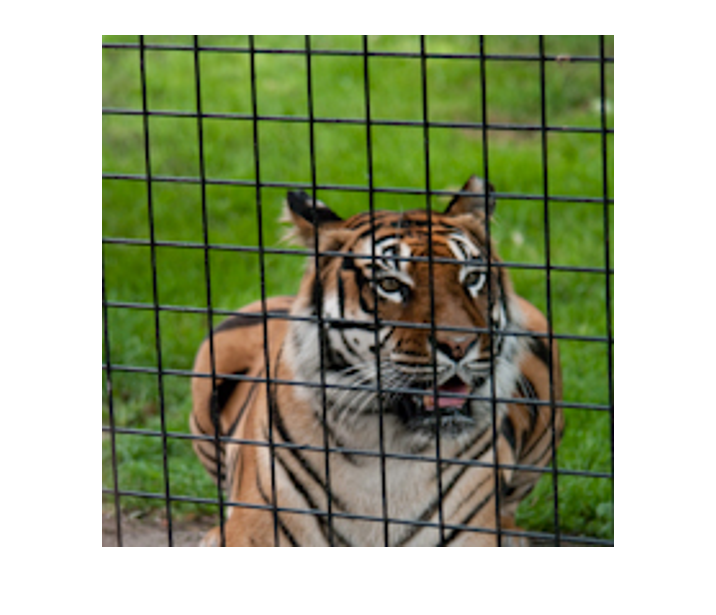
\includegraphics[width = .5\columnwidth]{fig/tigre_rescale.png} &
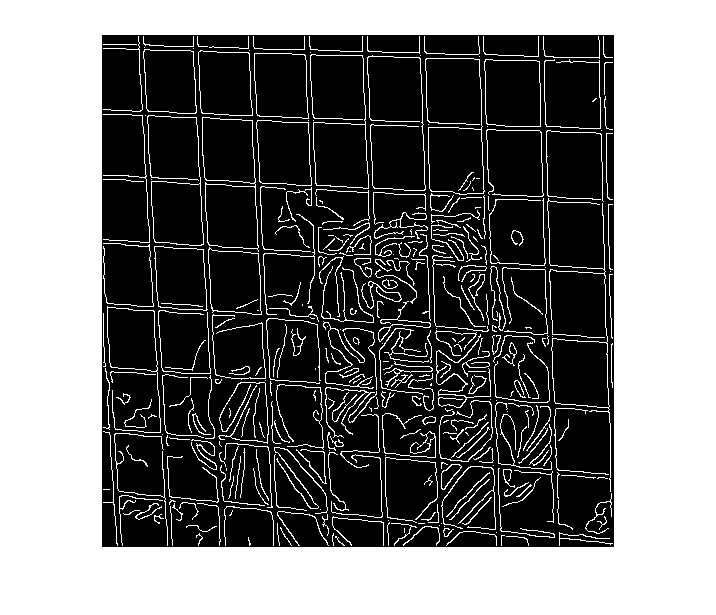
\includegraphics[width = .5\columnwidth]{fig/contour.png} \\
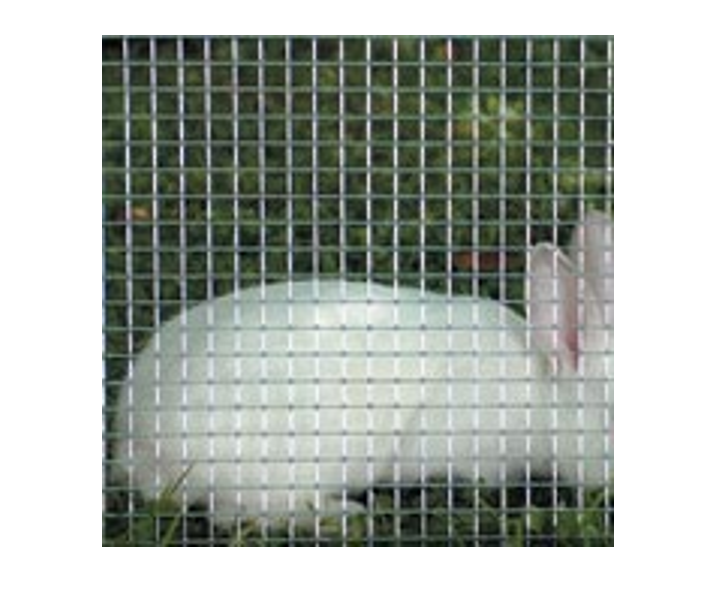
\includegraphics[width = .5\columnwidth]{fig/lapin_rescale.png} &
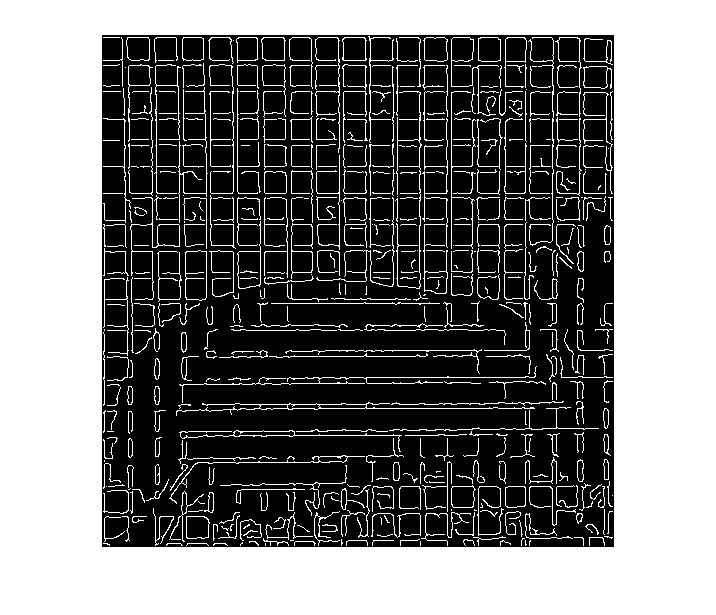
\includegraphics[width = .5\columnwidth]{fig/contour_lapin.png} \\
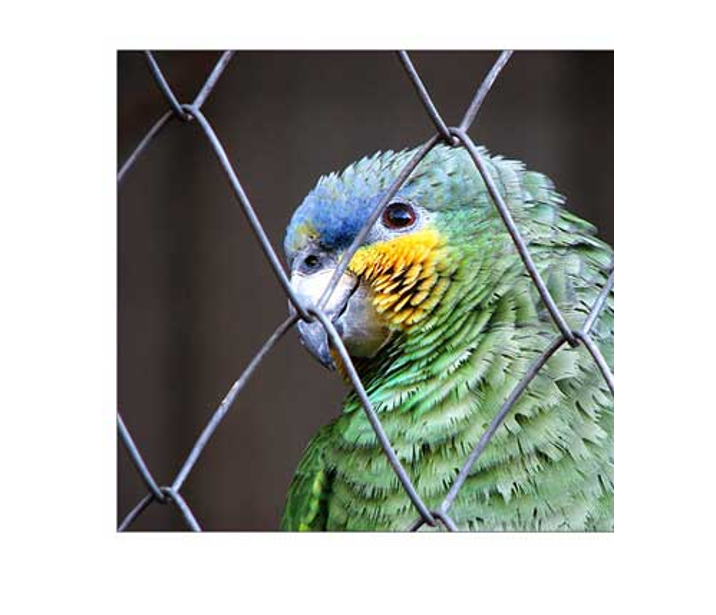
\includegraphics[width = .5\columnwidth]{fig/parrot_rescale.png} &
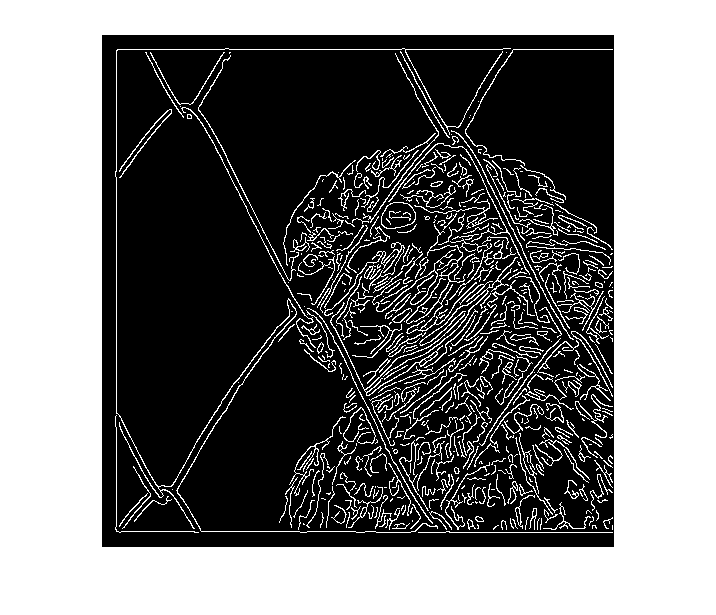
\includegraphics[width = .5\columnwidth]{fig/contour_parrot.png}
\end{tabular}
\caption{Dans les colonnes de gauche, l'image initiale et dans celles de droite les résultats de la détection de contour avec l'algorithme de Canny. Toutes les images sont redimensionnées en $512\times 512$. }
\label{fig101}
\end{figure}

\subsection{Extraction de lignes - transformation de Hough}

Nous ne rentrons pas dans les détails de la transformation de Hough mais en donnons ici plus une intuition qui nous sera utile pour plus tard. La transformation de Hough est une transformation qui permet d'extraire des droites d'une image. Le processus est représenté de manière graphique en Fig.(\ref{fig102}).

L'idée est de partir d'un point $A$ et de considérer toutes les droites passant par ce point. Ces droites sont paramétrées en coordonnées $(\rho,\theta)$ représentant respectivement l'angle et la distance - notons que sur un ordinateur, le point (0,0) est en haut à gauche et non en bas à gauche :
\begin{equation}
r = x \cos \theta + y \sin\theta
\end{equation}
Les droites passant par $A$ forment une sinusoïde dans l'espace d'arrivée. La droite passant par $A$ qui va passer par un autre point $B$ va également appartenir à la sinusoïde de $B$ dans l'espace image : elle sera représentée par un point à l'intersection des deux sinusoïdes. Pareil si cette même droite passe par un point $C$. C'est ainsi que si l'on alloue un compteur 1 à chaque sinusoïde d'un ensemble de points d'entrée, et que ce compteur est additif, alors trouver les maxima dans la transformation de Hough revient effectivement à extraire les lignes d'un nuage de points.

\begin{figure}[ht!]
\centering
\begin{tabular}{cc}
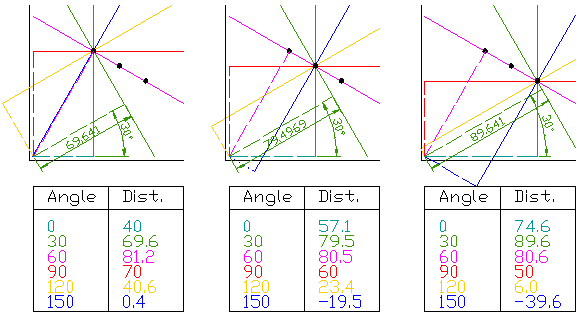
\includegraphics[width = .5\columnwidth]{fig/Hough_transform_diagram.png} &
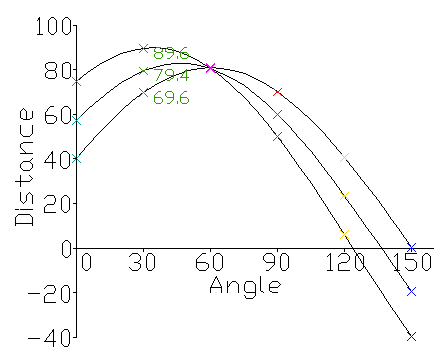
\includegraphics[width = .5\columnwidth]{fig/Hough_space_plot_example.png}
\end{tabular}
\caption{Transformation de Hough, les croisements dans l'espace arrivé correspondent aux droites dans l'image initiale. }
\label{fig102}
\end{figure}




\section{Identification d'un grillage}
\section{Reconstruction de l'image}

Une fois le masque appliqué à l'image, nous sommes ramené à un problème dit d'\emph{inpainting}. Il s'agit alors de trouver une méthode permettant de combler les trous formés par le masquage en respectant la structure de l'image. Il existe de nombreuses méthodes pour cela, nous en avons implémenté quelques unes. 

\subsection{Inpainting par régularisation variationnelle}

\subsubsection{Inpainting avec norme Sobolev}

La résolution du problème d'inpainting repose sur un problème de minimisation d'énergie - ici norme de Sobolev - sous des contraintes de correspondance. Ainsi si on note $Phi$ l'opérateur de masquage de l'image - avec le masque extrait - et $y$ l'image masquée, l'\emph{inpainting} par Sobolev se récrit :
\begin{equation}
f^* = \arg \min E(f) = \|\nabla f \|^2 \text{ sous contraintes } \Phi(f) = y
\end{equation}
Cette fonction à minimiser est régulière et l'on peut utiliser un algorithme de descente de gradient projeté. Si l'on note - $\Omega$ est le masque :
\begin{equation}
(\Pi f)_i = 
\left\{
\begin{array}{lll}
y_i & \text{si} & i\in\Omega \\
f_i & \text{si} & i\notin\Omega
\end{array}
\right.
\end{equation}
l'opérateur de projection orthogonal sur la contrainte $Phi f = y$, alors l'algorithme de descente de gradient projeté consiste à itérer : 
\begin{equation}
f^{(n+1)} = \Pi \left( f^{(n)} + \tau \Delta(f^{(n)})\right)
\end{equation}
où $\Delta = - \nabla^* \circ \nabla$ (l'adjoint du gradient étant -div. Le terme de mise à jour est donc bien le terme classique de gradient dans la descente de gradient - ici c'est le gradient de l'énergie de Sobolev $E(f)$. La condition de convergence de la méthode de descente de gradient projetée est que le pas de mise à jour vérifie : 
\begin{equation}
\tau < \frac{2}{\|\Delta \|}
\end{equation}

Les résultats de l'\emph{inpainting} avec norme de Sobolev sont présenté en figure (A FAIRE). INTERPRETATION.

 
\subsubsection{Inpainting avec norme TV}

On peut aussi remplacer dans le problème d'optimisation précédent la norme de Sobolev par la norme de variation totale (TV). Nous verrons qu'elle a tendance à mieux reconstruire les contours que la norme Sobolev qui floute les images. Pour autant elle n'est pas différentiable en 0, on lui préfère donc sa version régularisée :
\begin{equation}
J_{\epsilon}(f) = \sum_x \sqrt{\|\nabla f(x) \|^2 + \epsilon^2}
\end{equation}
De nouveau on peut réutiliser l'algorithme de descente de gradient projeté, il suffit donc de calculer le gradient de cette nouvelle énergie. Il vaut : 
\begin{equation}
G_{\epsilon} = - \text{div} \left( \frac{(\nabla f)_i}{\sqrt{\| (\nabla f)_i \|^2 + \epsilon^2}}\right)_i
\end{equation}
La contrainte à respecter sur le pas est cette fois-ci :
\begin{equation}
\tau < \frac{\epsilon}{4}
\end{equation}
(RESULTATS + INTERPRETATION).


\subsection{Inpainting par régularisation parcimonieuse}

Cette méthode d'\emph{inpainting} diffère de la première en ce sens qu'elle passe par une représentation parcimonieuse de l'image avant d'essayer de combler les trous. La représentation considérée est engendrée par une base de vecteurs $\Psi = (\psi_m)_m$, usuellement une base d'ondelette. Les coefficients dans cette base sont noté $a =(a_m)_m$, on par du principe que la représentation est parcimonieuse - \emph{i.e.} les $(a_m)_m$ le sont. On cherche un ensemble de coefficients $a^*$ qui résout :
\begin{equation}
a^* \in \arg \min_a \frac{1}{2} \| y - \Phi \Psi a \|^2 + \lambda J(a)
\end{equation}
Le paramètre $\lambda$ correspond à de la régularisation pour le bruit, comme nos images ne sont pas bruitée, nous prenons un $\lambda$ très faible. La notation $\Psi a = \sum_m a_m \psi_m$ indique uniquement l'opération de reconstruction du signal. Souvent on prend $J(a)$ comme la norme $L^1$ : $J(a) = \sum_m \|a_m \|$.

On note $S^{\Psi}(a)$ la fonction de seuillage - \emph{soft} ou \emph{hard} - dans la base $\Psi$. On peut prendre plusieurs bases d'ondelettes, nous présenterons des résultats pour une base orthogonale et une autre invariante par translation. L'algorithme utilisé pour résoudre le problème de minimisation précédent est le \emph{forward-backward splitting} - aussi connu comme \emph{iterative thresholding}. Il s'agit d'itérer : 
\begin{equation}
f^{(n+1)} = S^{\Psi}_{\tau,\lambda}(f^{(n)} - \tau \Phi^*(\Phi f^{(n)} - y) )
\end{equation}
L'avantage de prendre des ondelettes orthogonales est que $\Phi^* = \Phi$. Dans ce cas, pour qu'il y ait convergence le pas doit vérifier :
\begin{equation}
\tau < \frac{2}{\| \Phi^* \Phi \|} = 2
\end{equation}
Avec $\tau = 1$, et des ondelettes orthogonales toujours, l'étape de descente de gradient revient à projeter sur la contrainte $\mathcal{C} = \{f | \forall \Omega(x) = 1, f(x) = y(x) \}$. Ainsi dans le cas d'ondelettes orthogonales, l'algorithme revient à :
\begin{equation}
f^{(n+1)} = S_{\lambda}^{\Psi} (\text{Proj}_{\mathcal{C}} (f^{(n)}))
\end{equation}
Cet algorithme s'adapte dans le cas d'ondelette non orthogonales mais les dernières simplifications ne sont plus licites. 

(COMPARAISON METHODES + IMAGES).










\section*{Conclusion}




\newpage

\bibliographystyle{unsrt}
\bibliography{biblio}

\end{document}